\section{单纯映射诱导的同态}
\sourcepage{73--74}
若 $f$ 为从 $|K|$ 到 $|L|$ 的单纯映射，它把 $K$ 的每个 $p$ 维单形 $\sigma_i$ 映到 $L$ 的某个同维或低维单形 $\tau_i$ 上。下面定义 $p$ 维链之间的同态，把定向 $p$ 维单形的形式和 $\sum m_i\sigma_i$ 映到其像的形式和 $\sum m_i\tau_i$，删去后者中所有维数小于 $p$ 的 $\tau_i$。我们将看到，这个映射又诱导同调群之间的同态。

作为一般约定，“$f:K\to L$ 是单纯映射”表示：$f$ 是从 $|K|$ 到 $|L|$ 的连续映射，把 $K$ 的每个单形线性地映到 $L$ 的某个单形上。因此，它把顶点映到顶点，而且等于第 1.3 节所定义的由此顶点映射诱导的单纯映射。

\entry{定义}{1.13.1}设 $f:K\to L$ 为单纯映射。若 $v_0\cdots v_p$ 为 $K$ 的单形，则 $f(v_0),\ldots,f(v_p)$ 张成 $L$ 的单形。通过在定向单形上规定
\[
f_\#([v_0,\ldots,v_p])=
\begin{cases}
[f(v_0),\ldots,f(v_p)],&\text{若各 }f(v_i)\text{ 互异},\\
0,&\text{否则},
\end{cases}
\]
定义同态 $f_\#:C_p(K)\to C_p(L)$。它显然良定义：交换 $[v_0,\ldots,v_p]$ 中两个顶点，等式右边改变符号。在每个维数上各有一个这样的同态，它们组成的族 $\{f_\#\}$ 称为\textbf{单纯映射 $f$ 诱导的链映射}。

严格来说，应以维数下标区分这些同态，将 $p$ 维映射记为 $(f_\#)_p:C_p(K)\to C_p(L)$。通常像边界算子一样省略下标，由上下文说明。同样，为避免记号繁杂，也用 $\partial$ 同时表示 $K$ 与 $L$ 的边界算子；需要区分时可用 $\partial_K,\partial_L$。

\entry{引理}{1.13.2}同态 $f_\#$ 与 $\partial$ 可交换，因此诱导同态 $f_*:H_p(K)\to H_p(L)$。

\noindent\textbf{证明：}需要证明
\[
\partial f_\#([v_0,\ldots,v_p])=f_\#(\partial[v_0,\ldots,v_p]).\tag{$*$}
\]
设 $\tau$ 为 $f(v_0),\ldots,f(v_p)$ 张成的 $L$ 的单形，分情况讨论。

\textbf{情形一：}$\dim\tau=p$。这些像顶点互异，结论立即由 $f_\#$ 与 $\partial$ 的定义得到。

\textbf{情形二：}$\dim\tau\leq p-2$。由于像顶点不全互异，$(*)$ 左边为零。右边也为零，因为无论删去哪个 $f(v_i)$，余下点中至少仍有两个相同。

\textbf{情形三：}$\dim\tau=p-1$。不妨排序使 $f(v_0)=f(v_1)$，而 $f(v_1),\ldots,f(v_p)$ 互异。左边为零。右边许多项对应的像单形维数为 $p-2$，故这些项为零。仅有的两个非零项为
\[
[f(v_1),f(v_2),\ldots,f(v_p)]-[f(v_0),f(v_2),\ldots,f(v_p)],
\]
两者相互抵消，得到所需等式。

$f_\#$ 把闭链映为闭链，因为 $\partial c_p=0$ 蕴含 $\partial f_\#(c_p)=f_\#(\partial c_p)=0$；它也把边界映为边界，因为 $c_p=\partial d_{p+1}$ 蕴含 $f_\#(c_p)=f_\#(\partial d_{p+1})=\partial f_\#(d_{p+1})$。故它诱导同调群同态 $f_*$。\hfill$\square$

\sourcepage{75}
\entry{定理}{1.13.3}
\begin{enumerate}[label=(\alph*)]
\item 若 $i:K\to K$ 为恒等单纯映射，则 $i_*:H_p(K)\to H_p(K)$ 为恒等同态。
\item 若 $f:K\to L$、$g:L\to M$ 为单纯映射，则 $(g\circ f)_*=g_*\circ f_*$，即从 $H_p(K)$ 经 $H_p(L)$ 到 $H_p(M)$ 的复合，等于直接由 $g\circ f$ 诱导的同态。
\end{enumerate}
\noindent\textbf{证明：}由定义立即可验证，$i_*$ 为恒等映射，且 $(g\circ f)_*=g_*\circ f_*$。\hfill$\square$

这个定理表述了诱导同态的所谓“函子性质”。讨论范畴与函子时将正式定义此术语。现在只需指出：算子 $H_p$ 给每个单纯复形指定一个阿贝尔群，算子 $*$ 给每个单纯映射指定相应群之间的同态。因为 (a)、(b) 成立，称 $(H_p,*)$ 为从单纯复形与单纯映射的“范畴”到阿贝尔群与同态的“范畴”的一个“函子”。

\entry{引理}{1.13.4}链映射 $f_\#$ 保持增广映射 $\epsilon$，因此诱导约化同调群之间的同态 $f_*$。

\noindent\textbf{证明：}对 $K$ 的每个顶点 $v$，有 $\epsilon f_\#(v)=1=\epsilon(v)$，故 $\epsilon\circ f_\#=\epsilon$。因此 $f_\#$ 把 $\epsilon_K:C_0(K)\to\Z$ 的核映到 $\epsilon_L:C_0(L)\to\Z$ 的核中，诱导 $f_*:\widetilde H_0(K)\to\widetilde H_0(L)$。\hfill$\square$

\entry{例}{1.13.5}考虑图 1.13.1 的复形 $K,T$，底空间分别为圆周和环面。$H_1(K)\cong\Z$，取图中闭链 $z$ 为生成元。$H_1(T)\cong\Z\oplus\Z$，以
\[
w_1=[A,B]+[B,C]+[C,A],\qquad z_1=[A,D]+[D,E]+[E,A]
\]
的陪集为基。考虑下表指定的三个单纯映射：
\begin{center}
\begin{tabular}{c|ccc}
顶点&$f$&$g$&$h$\\\hline
$a$&$A$&$A$&$A$\\
$b$&$P$&$B$&$I$\\
$c$&$D$&$C$&$J$\\
$d$&$D$&$A$&$G$\\
$e$&$P$&$E$&$G$\\
$p$&$E$&$D$&$A$
\end{tabular}
\end{center}
可以验证，$f_\#(z)$ 同调于 $z_1$，$g_\#(z)=w_1-z_1$，而 $h_\#(z)$ 同调于 $w_1-z_1$。因此 $g_*,h_*$ 在一维同调上相同，在零维同调上也相同。
\begin{center}
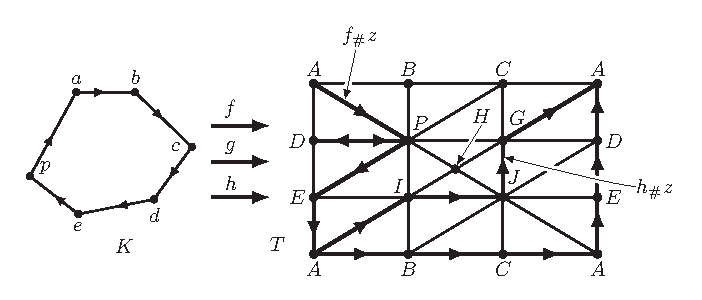
\includegraphics[width=121mm]{figures/1-13-1.pdf}\\图 1.13.1
\end{center}

\sourcepage{76--77}
如前例所示，很不相同的单纯映射也可以诱导同一个同态。因此要问：在什么条件下，两个单纯映射诱导同一个同调群同态？回答这个问题需要一种重要技巧，后文将多次使用，先解释其动机。

给定单纯映射 $f,g:K\to L$，希望找到条件，保证每个闭链 $z\in Z_p(K)$ 的像 $f_\#(z),g_\#(z)$ 同调。换言之，希望有一个通常记作 $D$ 的函数，为每条 $p$ 维闭链 $z$ 指定 $L$ 的一条 $(p+1)$ 维链 $Dz$，使
\[
\partial Dz=g_\#(z)-f_\#(z).
\]
考虑一个能做到这一点的例子。设 $K$ 为三角形区域的边界，$L$ 由图 1.13.2 的三棱柱侧面组成；$f,g$ 分别把 $K$ 映到棱柱的两端。若 $z$ 为图中生成 $H_1(K)$ 的闭链，很容易找到边界为 $g_\#(z)-f_\#(z)$ 的 $2$ 维链 $Dz$：取 $L$ 中所有适当定向的 $2$ 维单形之和即可。
\begin{center}
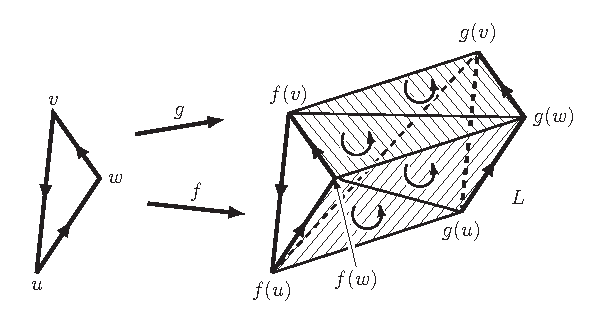
\includegraphics[width=105mm]{figures/1-13-2.pdf}\\图 1.13.2
\end{center}
一般地，只在闭链上定义 $D$ 很不方便，因为需要先计算闭链群。更好的办法是在整个链群上把 $D$ 定义为同态，这样可以逐个单形定义。在本例中如何做呢？给定顶点 $v$，定义 $Dv$ 为从 $f(v)$ 到 $g(v)$ 的边，如图 1.13.3。给定定向 $1$ 维单形 $\sigma$，定义 $D\sigma$ 为图中深色阴影的两个定向单形之和，它们组成棱柱的一个侧面。对其他单形也类似。由于 $z$ 是各定向边之和，$Dz$ 就是 $L$ 的所有定向 $2$ 维单形之和，仍满足所需等式。

对于任意链 $c$，$\partial Dc$ 满足什么公式？由定义即可看出。对定向单形 $\sigma$，由图 1.13.3 验证
\[
\partial D\sigma=g_\#(\sigma)-Dv-f_\#(\sigma)+Dw,
\]
即
\[
\partial(D\sigma)=g_\#(\sigma)-f_\#(\sigma)-D(\partial\sigma).\tag{$**$}
\]
对 $K$ 的其他单形也有相同公式。
\begin{center}
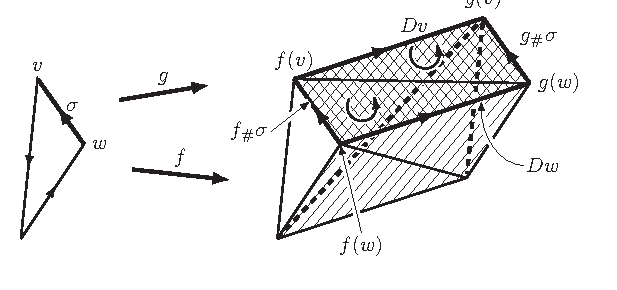
\includegraphics[width=105mm]{figures/1-13-3.pdf}\\图 1.13.3
\end{center}
这表述了同态 $D$ 的关键代数性质，正是我们所寻求的公式，将其纳入定义。

\sourcepage{78--79}
\entry{定义}{1.13.6}设 $f,g:K\to L$ 为单纯映射。若对每个 $p$ 都有同态 $D:C_p(K)\to C_{p+1}(L)$，满足
\[
\partial D+D\partial=g_\#-f_\#,
\]
则称 $D$ 为 $f_\#$ 与 $g_\#$ 之间的\textbf{链同伦}（chain homotopy）。

这里省略了维数下标。写出下标，公式为
\[
\partial_{p+1}D_p+D_{p-1}\partial_p=(g_\#)_p-(f_\#)_p,
\]
其中 $D_p:C_p(K)\to C_{p+1}(L)$，$D_{p-1}:C_{p-1}(K)\to C_p(L)$。这更精确，但记号繁杂，通常仍省略下标。

链同伦的重要性来自下列定理。

\entry{定理}{1.13.7}若 $f_\#$ 与 $g_\#$ 之间存在链同伦，则其诱导同态 $f_*,g_*$ 相等，对约化同调和普通同调都成立。

\noindent\textbf{证明：}若 $z$ 为 $p$ 维闭链，则
\[
g_\#(z)-f_\#(z)=\partial Dz+D\partial z=\partial Dz+0,
\]
所以两者属于同一同调类，即 $g_*(\{z\})=f_*(\{z\})$。\hfill$\square$

我们仍要寻找使 $f_*=g_*$ 的条件；现在已将问题归结为：在什么条件下可以构造 $f_\#,g_\#$ 之间的链同伦？下面给出一组条件。

\entry{定义}{1.13.8}若对 $K$ 的每个单形 $v_0\cdots v_p$，点
\[
f(v_0),\ldots,f(v_p),g(v_0),\ldots,g(v_p)
\]
张成 $L$ 的一个单形 $\tau$，则称单纯映射 $f,g:K\to L$ \textbf{邻接}（contiguous）。依互异点的个数，$\tau$ 的维数可为 $0$ 到 $2p+1$ 中的任一数。

粗略地说，这个条件表示 $f,g$ 相当接近：可以穿过某个可能较大的单形 $\tau$，把 $f(\sigma)$ 移到 $g(\sigma)$，而两者都是 $\tau$ 的面。

\entry{定理}{1.13.9}若 $f,g:K\to L$ 邻接，则 $f_\#,g_\#$ 之间存在链同伦。

\noindent\textbf{证明：}下面是一种标准论证，应当掌握。对于 $K$ 的每个单形 $\sigma=v_0\cdots v_p$，令 $L(\sigma)$ 为由顶点集
\[
\{f(v_0),\ldots,f(v_p),g(v_0),\ldots,g(v_p)\}
\]
张成的单形及其各面构成的子复形。注意：
\begin{enumerate}[label=(\arabic*)]
\item $L(\sigma)$ 非空，且对所有 $i$ 有 $\widetilde H_i(L(\sigma))=0$，见定理 1.9.7。
\item 若 $s$ 为 $\sigma$ 的面，则 $L(s)\subset L(\sigma)$。
\item 对每个定向单形 $\sigma$，链 $f_\#(\sigma),g_\#(\sigma)$ 都由 $L(\sigma)$ 承载。
\end{enumerate}
利用这些事实，对 $p$ 归纳构造 $D:C_p(K)\to C_{p+1}(L)$，使每条 $D\sigma$ 都由 $L(\sigma)$ 承载。

令 $p=0$，取顶点 $v$。因为 $f_\#,g_\#$ 保持增广，
\[
\epsilon(g_\#(v)-f_\#(v))=1-1=0.
\]
因此此差代表 $\widetilde H_0(L(v))$ 的元素。该群为零，可选取由 $L(v)$ 承载的 $1$ 维链 $Dv$，使 $\partial Dv=g_\#(v)-f_\#(v)$。于是 $\partial Dv+D\partial v=g_\#(v)-f_\#(v)$。对每个顶点如此定义 $D$。

现设在小于 $p$ 的维数已定义 $D$，使每个这样的定向单形 $s$ 满足 $Ds$ 由 $L(s)$ 承载，且 $\partial Ds+D\partial s=g_\#(s)-f_\#(s)$。给定定向 $p$ 维单形 $\sigma$，希望定义 $D\sigma$，使其边界等于
\[
c=g_\#(\sigma)-f_\#(\sigma)-D\partial\sigma.
\]
因为 $\partial\sigma$ 为 $p-1$ 维链，$D\partial\sigma$ 已定义，故 $c$ 良定义。它还是闭链：对 $\partial\sigma$ 用归纳假设，并利用 $\partial^2=0$，得
\[
\begin{aligned}
\partial c&=\partial g_\#(\sigma)-\partial f_\#(\sigma)-\partial D(\partial\sigma)\\
&=\partial g_\#(\sigma)-\partial f_\#(\sigma)
-\bigl[g_\#(\partial\sigma)-f_\#(\partial\sigma)-D\partial(\partial\sigma)\bigr]\\
&=\partial g_\#(\sigma)-\partial f_\#(\sigma)-g_\#(\partial\sigma)+f_\#(\partial\sigma)=0.
\end{aligned}
\]
\translatornote{原文展开式中有两处多印 $\partial$，成为 $\partial f_\#(\partial\sigma)$，维数不合；这里按链同伦恒等式写出计算。}
再验证 $c$ 由 $L(\sigma)$ 承载。由 (3)，前两项如此。$\partial\sigma$ 是定向面的和，每个面的像 $Ds$ 由 $L(s)$ 承载，而由 (2)，$L(s)\subset L(\sigma)$，故第三项也如此。

因为 $c$ 是由 $L(\sigma)$ 承载的 $p$ 维闭链，且 $H_p(L(\sigma))=0$，可选取同样由其承载的 $(p+1)$ 维链 $D\sigma$，使
\[
\partial D\sigma=c=g_\#(\sigma)-f_\#(\sigma)-D\partial\sigma.
\]
再定义 $D(-\sigma)=-D(\sigma)$。对每个 $p$ 维单形重复此过程，就得到 $p$ 维上所需的链同伦。定理得证。\hfill$\square$

\sourcepage{80--81}
有些学生对构造 $D$ 时必须作任意选择感到不安，希望有一个确定公式。遗憾的是，没有这样一个简洁公式。根本原因在于，$f_\#,g_\#$ 之间可能有许多链同伦，没有理由偏爱其中一个。

以特例说明。证明第一步中，若 $v$ 为顶点，则 $Dv$ 实际唯一确定：因为它必须由 $L(v)$ 承载，所以
\[
Dv=\begin{cases}0,&f(v)=g(v),\\\lbrack f(v),g(v)\rbrack,&f(v)\ne g(v).\end{cases}
\]
第一种情形 $L(v)$ 为顶点，第二种为一条边及其各面。

但下一步就可能有选择。设 $\sigma=vw$ 为边，$f(v),f(w),g(v),g(w)$ 互异，张成图 1.13.4 的 $3$ 维单形 $\tau$。图中给出了 $Dv,Dw$。如何定义 $D\sigma$？对于边界为图 1.13.5 所示 $g_\#(\sigma)-f_\#(\sigma)-D\partial\sigma$ 的 $2$ 维链，有两个明显选择：按图示定向取 $\tau$ 前面的两个面之和，或适当定向取后面的两个面之和。没有理由偏爱其中之一，只能任意选择。
\begin{center}
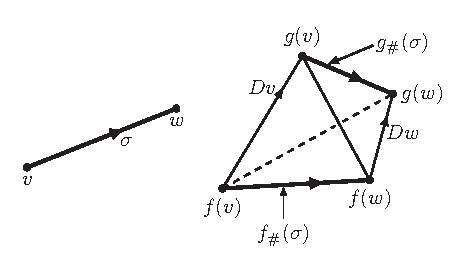
\includegraphics[width=85mm]{figures/1-13-4.pdf}\\图 1.13.4
\medskip

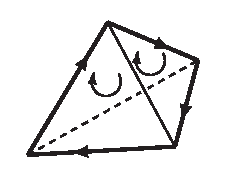
\includegraphics[width=43mm]{figures/1-13-5.pdf}\\图 1.13.5
\end{center}
\subsection*{在相对同调中的应用}
设 $K_0,L_0$ 分别为 $K,L$ 的子复形，单纯映射 $f:K\to L$ 将 $K_0$ 的每个单形映入 $L_0$ 的某个单形。常说“$f:(K,K_0)\to(L,L_0)$ 是单纯映射”。这时 $f_\#$ 将 $C_p(K_0)$ 映入 $C_p(L_0)$，诱导相对链映射
\[
f_\#:C_p(K,K_0)\to C_p(L,L_0).
\]
它与 $\partial$ 可交换，因此诱导同态 $f_*:H_p(K,K_0)\to H_p(L,L_0)$。定理 1.13.3 的函子性质立即推广到相对同调。

\entry{定义}{1.13.10}若 $f,g:(K,K_0)\to(L,L_0)$ 满足：对 $K$ 的每个单形 $\sigma=v_0\cdots v_p$，各点 $f(v_0),\ldots,f(v_p),g(v_0),\ldots,g(v_p)$ 张成 $L$ 的一个单形，且当 $\sigma\in K_0$ 时，它们张成 $L_0$ 的一个单形，则称 $f,g$ \textbf{作为偶的映射邻接}。

\sourcepage{82--84}
\entry{定理}{1.13.11}若 $f,g:(K,K_0)\to(L,L_0)$ 作为偶的映射邻接，则对所有 $p$ 存在同态 $D:C_p(K,K_0)\to C_{p+1}(L,L_0)$，满足 $\partial D+D\partial=g_\#-f_\#$。因此 $f_*,g_*$ 在相对同调群上相等。

\noindent\textbf{证明：}定理 1.13.9 构造的 $D$ 自动将 $C_p(K_0)$ 映入 $C_{p+1}(L_0)$：若 $\sigma\in K_0$，则 $L(\sigma)$ 按定义为 $L_0$ 的子复形，而 $D\sigma$ 由 $L(\sigma)$ 承载。因此 $D$ 诱导了相对链群间所需的同态。\hfill$\square$

\subsection*{习题}
\begin{enumerate}
\item 验证例 1.13.5 中的各项断言。
\item 考虑图 1.13.6 的顶点标记指定的复形 $K$，底空间为环面。虽与前面的复形略有不同，同调计算不变。令 $\gamma$ 为所有逆时针定向 $2$ 维单形之和，则它生成 $H_2(K)$。闭链 $w_1=[a,b]+[b,c]+[c,a]$、$z_1=[a,d]+[d,e]+[e,a]$ 生成 $H_1(K)$。
\begin{enumerate}[label=(\alph*)]
\item 定义 $K$ 到自身的单纯映射 $f,g,h,k$，使其满足下表：
\begin{center}\begin{tabular}{c|cccc}
顶点&$f$&$g$&$h$&$k$\\\hline
$a$&$a$&$a$&$d$&$p$\\
$b$&$d$&$c$&$p$&$q$\\
$c$&$e$&$b$&$q$&$d$\\
$d$&$c$&$d$&$d$&$u$\\
$e$&$b$&$e$&$d$&$b$
\end{tabular}\end{center}
\item 计算 $f_*,g_*,h_*,k_*$ 在同调类 $\{w_1\},\{z_1\},\{\gamma\}$ 上的值。
\end{enumerate}
\begin{center}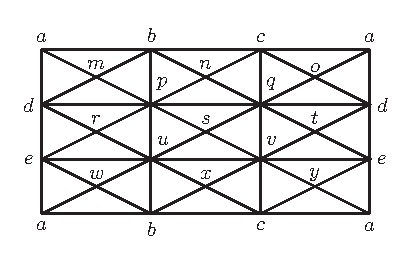
\includegraphics[width=76mm]{figures/1-13-6.pdf}\\图 1.13.6\end{center}
\item 用图 1.13.7 的复形表示 Klein 瓶 $S$，仍令 $w_1=[a,b]+[b,c]+[c,a]$、$z_1=[a,d]+[d,e]+[e,a]$。
\begin{enumerate}[label=(\alph*)]
\item 定义单纯映射 $f:S\to S$，使 $f_*(\{w_1\})=\{z_1\}$。
\item 证明不存在单纯映射 $g:S\to S$，使 $g_*(\{z_1\})=\{w_1\}$。
\end{enumerate}
\begin{center}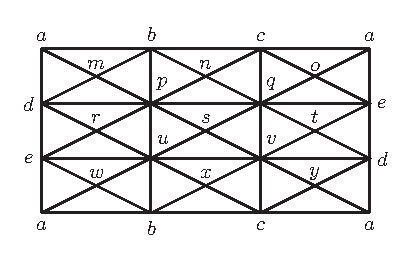
\includegraphics[width=76mm]{figures/1-13-7.pdf}\\图 1.13.7\end{center}
\item 设 $K$ 为习题 2 的环面，$\gamma$ 为其中的 $2$ 维闭链。设 $L$ 由顶点为 $A,B,C,D$ 的 $3$ 维单形的真面组成，令 $\gamma'=\partial[A,B,C,D]$，见图 1.13.8。
\begin{enumerate}[label=(\alph*)]
\item 证明从 $K$ 的顶点集到 $L$ 的顶点集的任意映射，都诱导 $K\to L$ 的单纯映射。
\item 令 $f$ 将 $m,r$ 映到 $A$，$p$ 映到 $B$，$b,u$ 映到 $C$，其他顶点均映到 $D$。用 $\gamma,\gamma'$ 表示诱导同态 $f_*:H_2(K)\to H_2(L)$。
\item 设 $g$ 在除 $r$ 外的顶点上与 $f$ 相同，而 $g(r)=C$，计算 $g_*$。
\item 设 $h$ 在除 $u$ 外的顶点上与 $g$ 相同，而 $h(u)=A$，计算 $h_*$。
\end{enumerate}
\begin{center}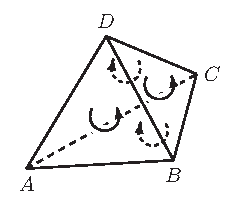
\includegraphics[width=43mm]{figures/1-13-8.pdf}\\图 1.13.8\end{center}
\item 设 $f,g:(K,K_0)\to(L,L_0)$ 为单纯映射。证明：若 $f,g$ 作为 $K\to L$ 的映射邻接，且 $L_0$ 是 $L$ 的满子复形，则它们作为偶的映射邻接，见定义 1.4.11。
\end{enumerate}
